\documentclass{article}
\usepackage[margin=2.5cm, top=4cm, headheight=25pt]{geometry}
\usepackage{amsmath, amssymb, enumitem, fancyhdr, graphicx}
\usepackage[indent=20pt]{parskip}
\usepackage[hidelinks]{hyperref}
\usepackage{xcolor}
\usepackage{listings}
\usepackage{subcaption}
\usepackage{url}
\usepackage[most]{tcolorbox}
\usepackage{lastpage}
\usepackage{tikz}
\usepackage{circuitikz}

\usetikzlibrary{arrows, positioning}
\tcbuselibrary{listingsutf8} % Support for lstlistings within tcolorbox

\newtcolorbox[auto counter, number within=section]{question}[1][]{%
    colframe=gray!80,                      % Dark gray frame
    colback=gray!5,                       % Light gray background
    coltitle=black,                        % Black title
    title=\textbf{Question~\thetcbcounter}, % Bold title
    fonttitle=\bfseries\large,             % Subtle title font size
    rounded corners,                   % Slightly more rounded corners
    boxrule=0.25mm,                         % Thinner border for a sleek look
    enhanced,                              % Enhanced box features
    attach boxed title to top left={xshift=2mm, yshift=-2mm},
    boxed title style={colframe=gray!80, colback=gray!5, boxrule=0.25mm},
    % Title styling
    #1
}

\bibliographystyle{IEEEtran}
\graphicspath{{./images/}}

% -- Custom Variables --
\def\me{Rajdeep Gill 7934493}
\def\course{ECE 3760}
\def\labsection{A01}

\def\labno{13}
\def\title{Assignment 13: Kalman Filter Estimation}
% -- Styling for code snippets --
\lstset{
    basicstyle=\ttfamily\scriptsize,           % Basic font style
    keywordstyle=\color{blue},            % Keywords color
    commentstyle=\color{gray},            % Comments color
    stringstyle=\color{teal},             % Strings color
    numbers=left,                         % Line numbers on the left
    numberstyle=\tiny\color{gray},        % Line number style
    stepnumber=1,                         % Line number step
    numbersep=10pt,                       % Space between line numbers and code
    backgroundcolor=\color{lightgray!10}, % Background color
    frame=single,                         % Adds a frame around the code
    breaklines=true,                      % Line breaking for long lines
    captionpos=b,                         % Caption position
    showspaces=false,                     % Don't show spaces
    showstringspaces=false                % Don't show spaces in strings
}
\renewcommand{\lstlistingname}{Code Snippet}

\renewcommand{\arraystretch}{1.2} % For less-ugly tables
\setlength\parindent{0pt}

%----- Samples 
% Questions:
%   \begin{question}[title=Custom Question Title]
%       Question details
%   \end{question}

% Tables:
%   \begin{table}[htbp]
%       \centering
%       \caption{Table Caption}
%       \begin{tabular}{ll}
%           \toprule
%           \textbf{Column 1} & \textbf{Column 2} \\
%           \midrule
%           Row 1 & Row 2 \\
%           Row 3 & Row 4 \\
%           \bottomrule
%       \end{tabular}
%   \end{table} 

% Figures:
%   Single figure:
%       \begin{figure}[htbp]
%           \centering
%           \includegraphics[width=0.5\textwidth]{example-image}
%           \caption{Figure Caption}
%       \end{figure}
%   Multiple figures:
%       \begin{figure}[htbp]
%           \centering
%           \begin{subfigure}[b]{0.5\textwidth}
%               \includegraphics[width=\textwidth]{example-image-a}
%               \caption{First subfigure}
%           \end{subfigure}
%           \begin{subfigure}[b]{0.5\textwidth}
%               \includegraphics[width=\textwidth]{example-image-b}
%               \caption{Second subfigure}
%           \end{subfigure}
%           \caption{Main figure}
%       \end{figure}

\begin{document}

% --------------------------------------------------------------------------------
% TITLE
% --------------------------------------------------------------------------------

\begin{center}
    \huge \title

    \vspace{2mm}
    \hrule

    \vspace{4mm}
    \large \me

    \vspace{2mm}
    \large \course~\labsection

    \vspace{2mm}
    \today
\end{center}

\vspace{4mm}

% --------------------------------------------------------------------------------
% END TITLE
% --------------------------------------------------------------------------------

\newpage


\vspace{1cm}
\newpage

\pagestyle{fancy}
\fancyhead[L]{\large Assignment \labno}
\fancyhead[R]{\large \me}

\fancyfoot[C]{Page \thepage~of~\pageref{LastPage}}

% --------------------------------------------------------------------------------
% BODY
% --------------------------------------------------------------------------------
\section{Kalman Filter Estimation}

We are given that the stride is 1 meter with a standard deviation of 0.2 meters, and variance of 0.04 meters. The PDF of one single stride is given by the following normal distribution:
\begin{align*}
    x &\sim \mathcal{N}(\mu, \sigma^2) \\
    \mu &= 1 \text{ m}, \quad \sigma^2 = 0.04 \text{ m}^2 \\
    \implies x &\sim \mathcal{N}(1, 0.04)
\end{align*}

Extending this to 100 steps, assuming one step is independent of the other, we can find the new mean and variance. The mean and variance of the sum of independent random variables is given by:
\begin{align*}
    \mu_{100} &= \sum_{i=1}^{100} \mu_i = 100 \\
    \sigma^2_{100} &= \sum_{i=1}^{100} \sigma^2_i = 100 \cdot 0.04 = 4
\end{align*}

Therefore, the PDF of 100 steps is given by:
\begin{align*}
    x_{100} &\sim \mathcal{N}(\mu_{100}, \sigma^2_{100}) = \mathcal{N}(100, 4) \\
\end{align*}

The two PDFs are shown in Figure \ref{fig:pdfs}.
\begin{figure}[ht!]
    \centering
    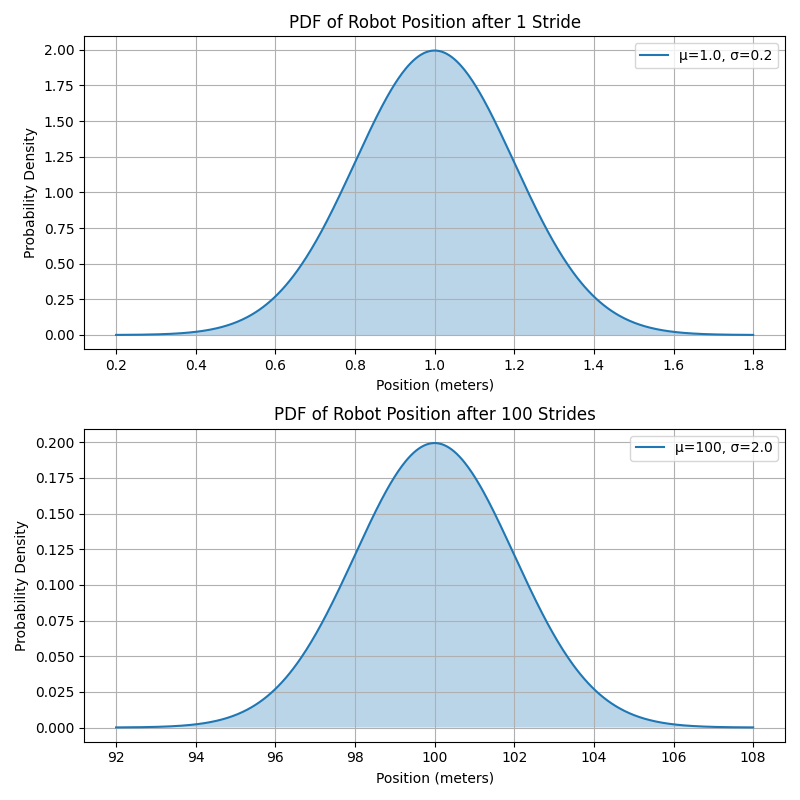
\includegraphics[width=0.5\textwidth]{pdf_plots.png}
    \caption{PDF of 1 step and 100 steps}
    \label{fig:pdfs}
\end{figure}

Utilizing a second input, which estimates a position of 105 meters with variance 1, the resultant fused PDF is as seen in Figure \ref{fig:pdfs_fused}. The mean and variance of the fused PDF is given by the following equations:
\begin{align*}
    \mu_{fused} &= \frac{\mu_{100}\cdot \sigma^2_{\text{sensor}} + \mu_{\text{sensor}} \cdot \sigma^2_{100}}{\sigma^2_{100} + \sigma^2_{\text{sensor}}} = \frac{100 \cdot 1 + 105 \cdot 4}{4 + 1} = \frac{520}{5} = 104 \\
    \sigma^2_{fused} &= \frac{\sigma^2_{100} \cdot \sigma^2_{\text{sensor}}}{\sigma^2_{100} + \sigma^2_{\text{sensor}}} = \frac{4 \cdot 1}{4 + 1} = \frac{4}{5} = 0.8
\end{align*}

Plotting this distribution over the previous two distributions, we can see that the position estimate is now more closer to the sensor input, and the variance is smaller than before. 
\begin{figure}[ht!]
    \centering
    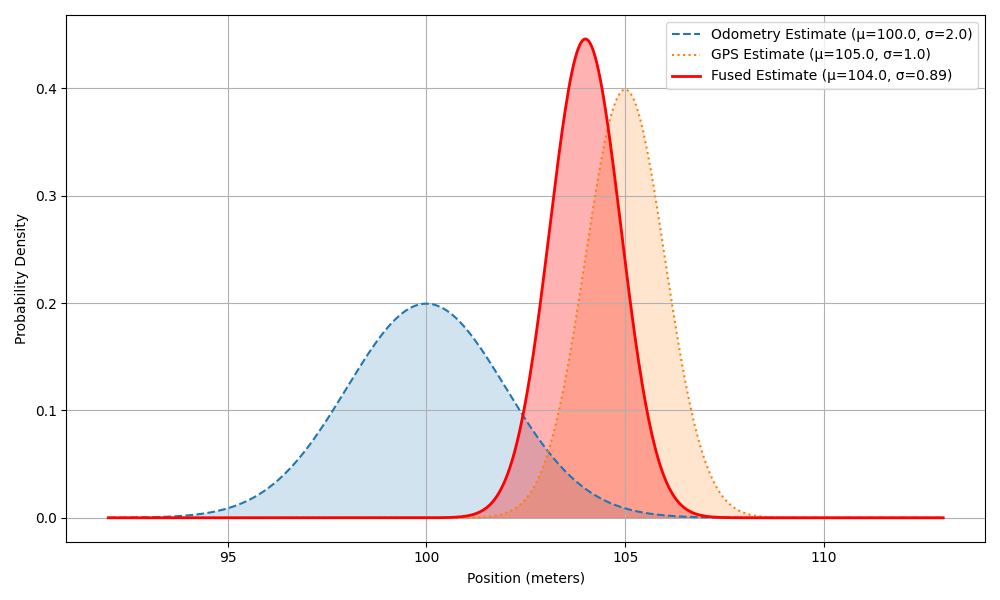
\includegraphics[width=0.5\textwidth]{fused_estimate_plot.png}
    \caption{Fused PDF of 100 steps and sensor input}
    \label{fig:pdfs_fused}
\end{figure}

% --------------------------------------------------------------------------------
% END BODY
% --------------------------------------------------------------------------------

\end{document}
